\section{Current mirror}
The circuit shown in Figure 11.1 is known as a current mirror circuit. First, students do
some theoretical calculations to get an understanding of it. After that, perform a simulation to double-check its principles and your analysis. Assume that the two transistors \(Q_1\)
and \(Q_2\), are the same type and the current gain \(\beta = 100\).

\begin{figure}[ht]
    \centering
    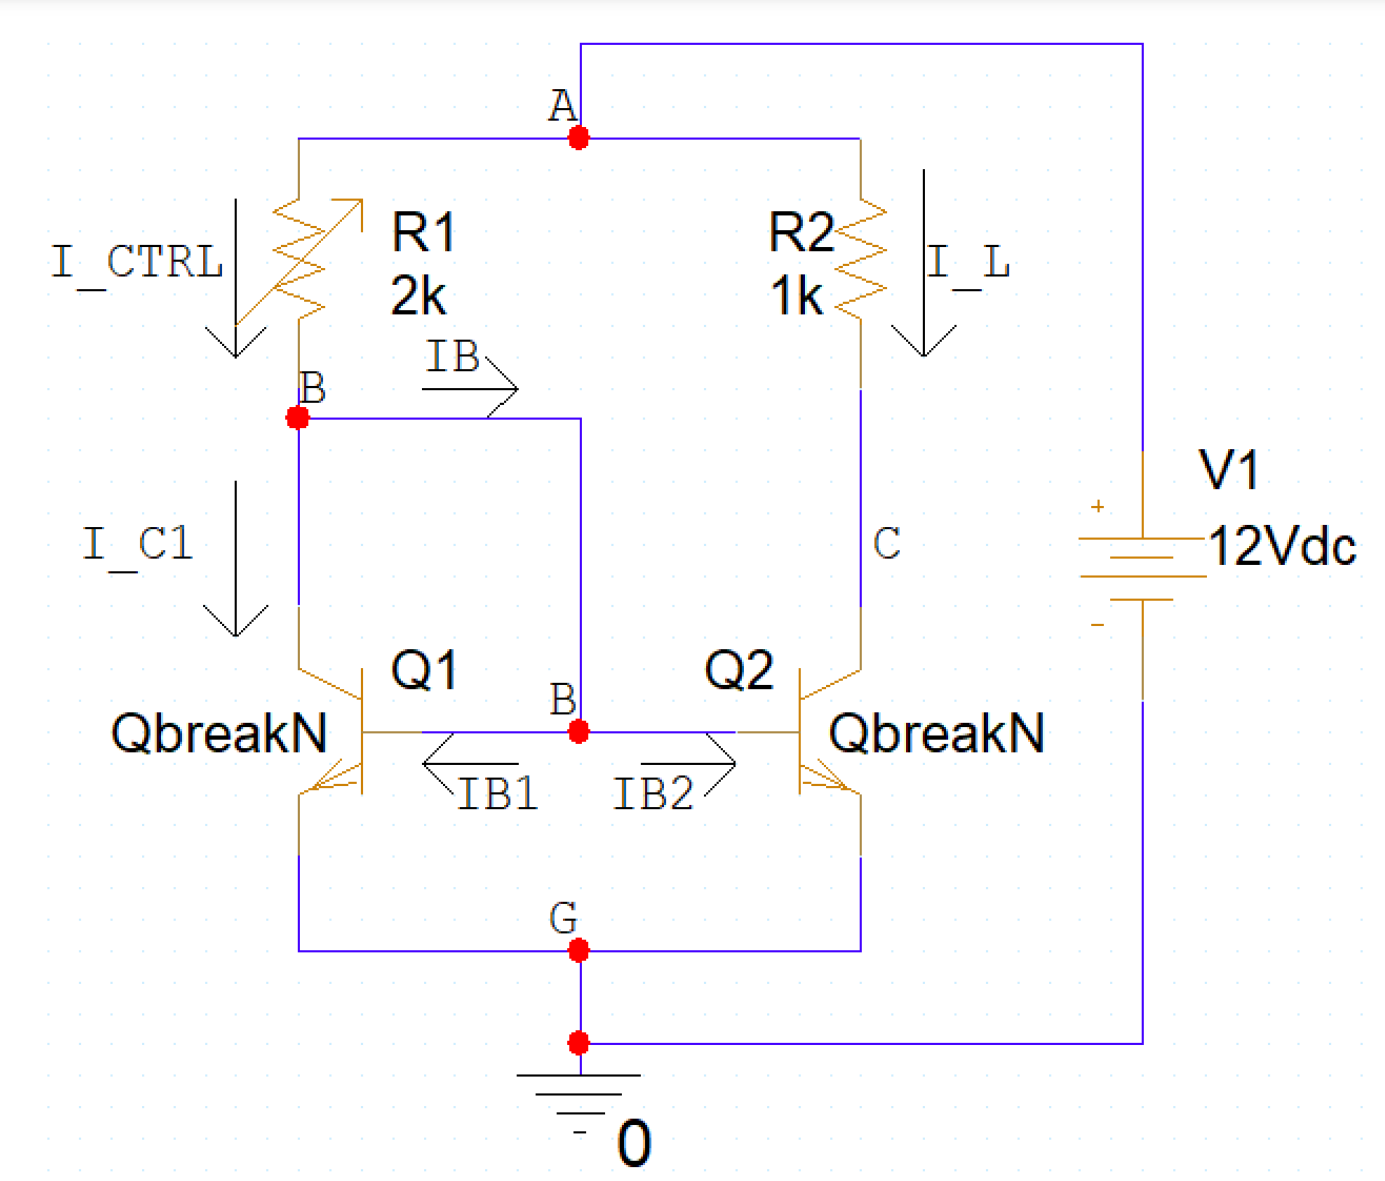
\includegraphics[scale=0.3]{graphics/ex11/f1.png}
    \caption{Current mirror circuit example}
\end{figure}

\subsection{Tính toán lí thuyết}

\textbf{Ghi chú:}

\textit{Những giải thích, công thức và phương trình được mong đợi hơn là chỉ có kết quả.}

Giả sử 2 transistors \(Q_1\) và \(Q_2\) trong vùng tích cực: \(V_{BG} \approx 0,7 V \)

Ta có: \(V_{BE} = V_B - V_G = 0,7\) V

 Mà \(V_G = 0\) V (Vì G nối đất)

 \( \implies V_B = 0,7\) V

 Ta có: \(V_{AG} = V_1 = V_A - V_B = 12 \) V hay \(V_A = 12\) V

 Theo Định luật Ohm, \(I_{CTRL} = \dfrac{V_A - V_B}{R_1} = \dfrac{12 - 0,7}{2.10^3} = 5,65 \) (mA)

 Theo KCL tại nút B, ta có: \(I_{CTRL} = I_{C1} + I_B = I_{C1} + I_{B_1} + I_{B_2}\) (1)

 Mà \(I_{B_1} = I_{B_2}\), \(I_{C1} = \beta I_{B_1}\) và \(I_{L} = \beta I_{B_2}\)
 
 \(\implies I_{C1} = I_L = 100I_{B_1} = 100I_{B_2}\) (2)

 Từ (1) và (2), ta có: \(I_{CTRL} = I_{C1} + 2I_{B_1} = 102I_{B_1}\)

 \(\iff I_{B_1} = I_{B_2} = \dfrac{I_{CTRL}}{102} \approx 0,05539 \) (mA)

 \(\implies I_{C1} = I_L = 100I_{B_1} \approx 5,539\) (mA)

 \subsection{Mô phỏng}
 
 \begin{figure}[ht]
    \centering
    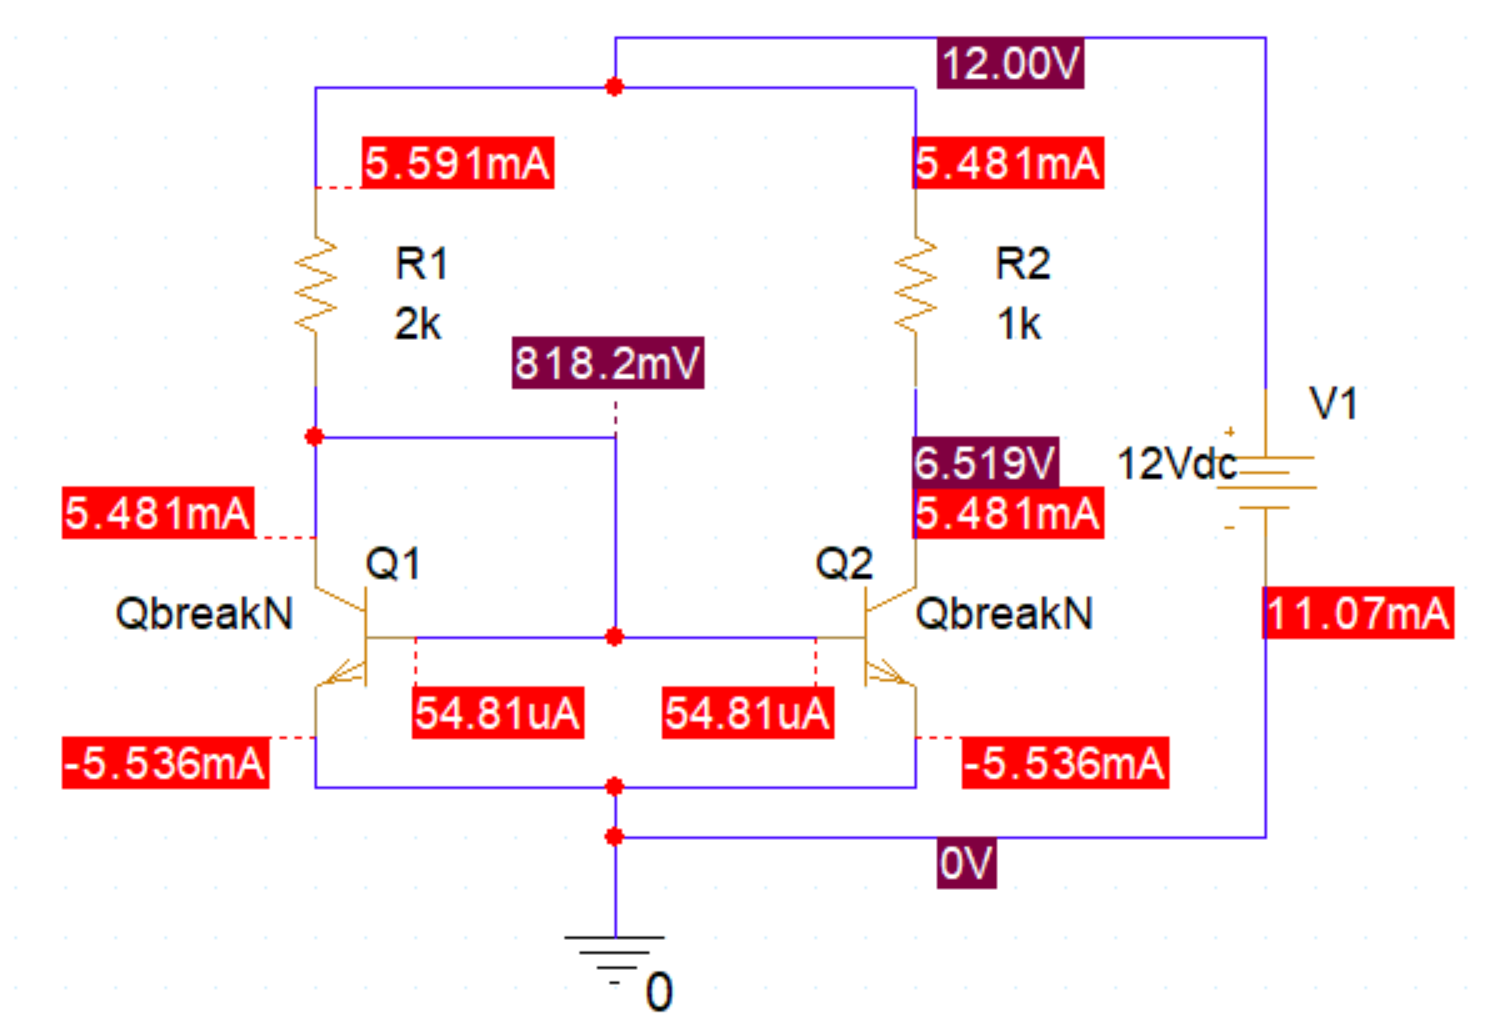
\includegraphics[scale=0.3]{graphics/ex11/f2.png}
    \caption{Simulation current mirror circuit example}
\end{figure}

Tại sao mạch trong Hình 11.1 được gọi là circuit mirror?

Vì trong trường hợp giá trị của \(R_2\) giới hạn trong vùng để transistors trong vùng tích cực, giá trị \(I_L\) không phụ thuộc vào giá trị của \(R_2\)
mà phụ thuộc vào giá trị của \(I_{C1}\). Cụ thể, \(I_L\) luôn luôn bằng với \(I_{C1}\) hay dòng điện tại đầu ra cực emitter của transistors Q1 
có giá trị luôn bằng với dòng điện tại đầu ra cực emitter của transistors Q2. Điều này giống như việc sao chép dòng điện \(I_{C1}\) thành dòng dòng điện \(I_{L}\).

 Bây giờ, thay thế điện trở \(R_1\) bằng điện trở 100 Ohms. Tiếp theo, tính toán lại tất cả các giá trị.
 Sau đó, cuối cùng, mô phỏng mạch mới và giải thích hiện tượng bạn đã quan sát được.

Giả sử transistors \(Q_1\) trong vùng tích cực, \(V_{BG} \approx 0,7\) V

Giống như trên ta cũng suy ra được \(V_A = 12\) V và \(V_B = 0,7\) V.

 Theo Định luật Ohm, \(I_{CTRL} = \dfrac{V_A - V_B}{R_1} = \dfrac{12 - 0,7}{100} = 113 \) (mA)

 Nếu transistors \(Q_2\) trong vùng tích cực
 
 Ta dùng lại kết quả từ (1) và (2), ta có: \(I_{CTRL} = I_{C1} + 2I_{B_1} = 102I_{B_1}\)

 \(\iff I_{B_1} = I_{B_2} = \dfrac{I_{CTRL}}{102} \approx 1,1078 \) (mA)

 \(\implies I_{C1} = I_L = 100I_{B_1} \approx 110,78\) (mA)
 
Nhưng \(V_{AG} = V_{AC} + V_{CG} = 12 \iff V_{CG} = V_{AG} - V_{AC} = 12 - 110,78.1 = -98,78 < 0\) (Điều này sai với transistors Q2 khi trong vùng tích cực) 

\(\implies \) \(Q_2\) bão hòa \(\implies V_{CG} \approx 0 \)

\(\implies I_L = I_{L_{(sat)}} \approx \dfrac{V_{AG}}{R_2} = \dfrac{12}{10^3} = 12 \) (mA)

Theo KCL tại nút B, ta có: \(I_{CTRL} = I_{C1} + I_{B1} + I_{B2} = 100I_{B1} + I_{B1} + I_{B2} = 113\) (mA)

\(\iff I_{B1} = I_{B2} = \dfrac{I_{CTRL}}{102} \approx 1,108 \) (mA)

\(I_{C1} = 100I_{B1} = 110,8\) (mA)

\textbf{Kết quả mô phỏng 2}

\begin{figure}[ht]
    \centering
    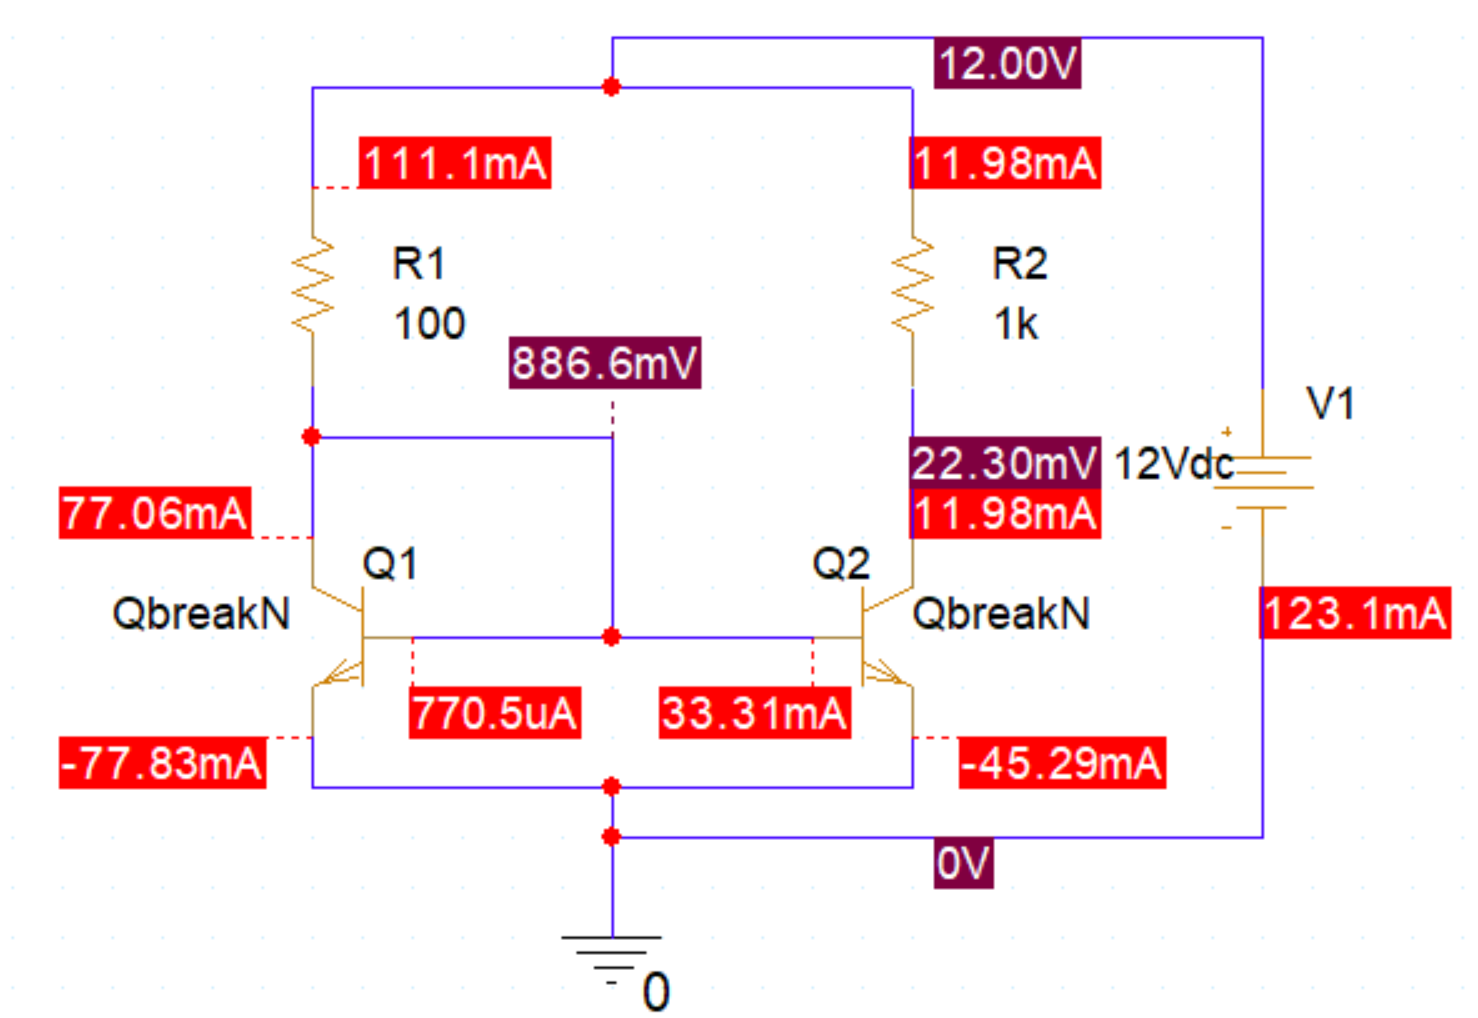
\includegraphics[scale=0.3]{graphics/ex11/f3.png}
    \caption{Simulation current mirror circuit example with \(R_1 = 100 \Omega\)}
\end{figure}

Hiện tượng gì xảy ra?

Kết quả tính toán theo lí thuyết không trùng khớp với kết quả mô phỏng.

Giải thích:

Thứ nhất, các giá trị đã giá định trong lí thuyết hoàn toàn khác so với mô phỏng (\(V_{BG} \approx 0,886 V, V_{CG} \approx 0,02 V\)) do đó mà giá trị của \(I_L, I_{CTRL}\) có chút sai lệch.

Thứ hai, trong mô phỏng ta thấy dòng \(I_{B1} \neq I_{B2}\). Điều này được cho là do trạng thái hoạt động transistors Q2 là bão hòa (khếch đại mạnh) trong khi Q1 hoạt động khếch đại , điều này dẫn đến khả năng cản trở dòng 
trở nên khác nhau. Do vậy, mạch không hoạt động như chúng ta tính toán được.

\pagebreak


 